%in Grundlagen
Operationsverstärker (kurz 'OPV oder 'OpAmp') dienen grundlegend der Verstärkung von 
Gleichspannungen. Sie besitzen einen nicht-invertierenden, der meist mit einem 
Plus, und einen invertierenden Eingang, der mit einem Minus dargestellt wird. Zu 
beachten ist, dass die Verstärkung auf die Differenzspannung der beiden Eingänge 
wirkt. Je zwei zusätzliche Anschlüsse finden sich für die positive und negative 
Betriebsspannung und für den Offsetabgleich, damit bei keiner Eingangsspannung 
auch keine Ausgangsspannung auftritt - dieser wird also in einer externen 
Schaltung durchgeführt.

\begin{figure}[H]
    \centering
    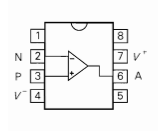
\includegraphics[width=6cm, height=6cm,keepaspectratio]{./figures/pics/pins.PNG}
    \caption{Schematische Darstellung der Pinbelegung eines klassischen Operationsverstärkers. Hierbei bezeichnet 2 den invertierenden, 3 den nicht invertierenden Eingangskanal, 6 den Ausgang, 4 den Anschluss für die negative sowie 7 den Anschluss für die positive Betriebsspannung, 1 und 5 die Pins für den Offserabgleich und 8 einen freien Pin.  \cite{tietze}}
    \label{fig:pin_anschl}
\end{figure}

In \autoref{fig:pin_anschl} sind die Pins eines Operationsverstärkers, wie er auch 
in der Laborübung verwendet wurde, zu sehen. Dabei ist zu beachten, dass jeder nicht 
belegte Pin auf Masse gelegt werden soll.

Es gibt vier grundlegende Arten der Verwendung von Operationsverstärkern, darunter
der nicht-invertierende Betrieb, bei dem das Eingangssignal nur auf den nicht-invertierenden 
Kanal gelegt wird und der invertierende auf Masse gelegt wird. Analog funktioniert der invertierende 
Modus, bei dem das Signal nun an den invertierenden Eingang gelegt wird, wodurch die Ausgangsspannung 
zusätzlich zur Verstärkung noch zum Eingangssignal invertiert wird. Beim Differenzbetrieb werden an 
beide Eingänge Signale angelegt und die Differenzspannung verstärkt. Im Falle des Gleichtaktbetriebs 
liegt das gleiche Eingangssignal an den beiden Eingängen an, wodurch es theoretisch keine Differenzspannung 
und Verstärkung geben sollte - in der Realität resultiert allerdings eine Verstärkung, die als 
Gleichtaktverstärkung bezeichnet wird.

Da der Operationsverstärker ohne zusätzliche Verkopplung sehr stark frequenzabhängig ist und 
nur eine geringe Bandbreite gewünscht verstärkt, wird eine Gegenkopplung vom Ausgang zum Eingang 
durchgeführt, wodurch die Verstärkung zwar abnimmt, die Bandbreite jedoch stark vergrößert wird. 
Die Bandbreite wird wie gewohnt durch die Grenzfrequenz chraktersisiert, bei welcher die Verstärkung 
noch \SI{70}{\%} der maximalen beträgt. Wenn nun beispielsweise ein Kondensator in der Rückkopplung verbaut wird, 
handelt es sich um eine Integratorschaltung, die im zweiten Teil der Laborübung untersucht wird.

Die resultierende Verstärkung lässt sich gemäß \autoref{eq:ver} als Verhätlnis der Ausgangs- $U_a$ zur Eingangsspannung $U_e$ berechnen.
\begin{equation}
	V=\frac{U_a}{U_e}
	\label{eq:ver}
\end{equation}
